%Fragen an Lehmann
%Soll ich noch Literatur dazu ein binden?
%Welchen Controller könnte ich verwenden?

\chapter{Batterie}\label{introduction}
Die Kernkomponente dieser Arbeit wird der Bau der Batterie sein, die den Motor des E-Bikes antreiben wird.
Hierbei werde ich größere Lithium-Ionen-Zellen verwenden und diese in einer geeigneten Konfiguration zusammenschließen, um die benötigte Spannung und Kapazität zu erreichen.
Zudem wird ein Smart Battery Management System (BMS) eingesetzt, um die Sicherheit und Effizienz der Batterie zu gewährleisten.\\

Des Weiteren liegt im Fokus die Programmierung des Controllers.
Ich will die Motordaten und die Leistung flexibel anpassen, um das E-Bike sowohl Straßen tauglich zu machen (maximale Leistung 250W), als auch zu testen, welche Leistung ein 1500W Motor erreicht (bringt) (auf einem Privatgrundstück).\\


Eine essenzielle Komponente bei der Realisierung eines individuell konstruierten E-Bikes ist die Batterie, welche den Motor mit der benötigten Energie versorgt.
Im vorliegenden Abschnitt wird detailliert auf die Fertigung einer individuellen Lithium-Ionen-Batterie eingegangen, die durch die Auswahl passenden Zellen und ihre spezifische Konfiguration realisiert wird.\\

%Was muss die Batterie Leisten?
Die Batterie muss den spezifizierten Anforderungen hinsichtlich Leistung, Form und Stabilität entsprechen.
In Bezug auf die Leistung ist eine Spannung von 48 Volt erforderlich, um den Motor zu versorgen.
Damit die gewünschte Leistung gewährleistet wird, muss die Batterie eine Leistung von 1500 Watt bereitstellen.
Eine Berechnung erfolgt mit nachfolgender Formel~\ref{eq:wattformel}:
\begin{equation}
    P = U \cdot I \longrightarrow I = \frac{P}{U}= \frac{1500W}{48V}= 31.25
    \label{eq:wattformel}
\end{equation}
\label{introduction2}
%Welche Kapazität soll die Batterie haben?

Die Batterie sollte nicht nur die erforderliche Leistung liefern, sondern auch eine stabile und sichere Form aufweisen.
Die physikalische Stabilität der Batterie ist entscheidend, um sicherzustellen, dass sie den Belastungen während des Betriebs standhält und keine strukturellen Schwächen aufweist.\\

Darüber hinaus ist die Form der Batterie relevant, da sie in das E-Bike integriert werden muss.
Die Form sollte daher kompatibel mit dem vorgesehenen Platzierungsort sein, um eine effiziente Nutzung des verfügbaren Raums zu ermöglichen.
Damit eine optimale Integration in das Gesamtsystem gewährleistet ist, ist eine leichte und sichere Befestigung des Akkus im vorgesehenen Bereich erforderlich.
Die Konstruktion der Batterie stellt einen maßgeblichen Schritt im Bau eines selbst gefertigten E-Bikes dar, da sie maßgeblich die Leistung und Reichweite des Fahrzeugs beeinflusst.


\section{Zellen}
%Welche Rollen spielen die Zellen im Batterie bau?
Die Zellen in einer Lithium-Ionen-Batterie für E-Bikes spielen eine entscheidende Rolle bei der Speicherung und Bereitstellung elektrischer Energie.
Jede Zelle fungiert als eigenständige Energieeinheit, welche miteinander kombiniert wird, um die gewünschte Spannung und Kapazität für den E-Bike-Motor zu erreichen.
Ihre Aufgaben umfassen die Speicherung von Elektronen während des Ladevorgangs und die Abgabe dieser Elektronen während des Entladevorgangs, um den Motor mit Strom zu versorgen.\\

%Wie werden sie verbunden?
Die Zellen werden in der Batterie durch spezifische Verbindungsmethoden miteinander verbunden.
Die Verbindung erfolgt durch das serielle Schalten der Zellen, wodurch die Einzelspannungen addiert werden.
Dieser Schritt ermöglicht es, die für den E-Bike-Motor erforderliche höhere Gesamtspannung von 48 Volt zu erreichen.
Wie viele Zellen in Reihe geschaltet werden müssen um auf 48V zukommen, wird hier berechnet:~\ref{eq:Strom}\\
%Wie ist der schaltplan?
Die Entscheidung, Zellen in Serie oder parallel zu schalten, beeinflusst maßgeblich die Leistung und Charakteristik der Batterie.
Die Reihenschaltung erhöht die Gesamtspannung, während die Parallelschaltung die Gesamtkapazität steigert.
Dadurch wird eine direkte Auswirkung auf die Leistungsfähigkeit des E-Bikes erzielt.\\

\subsection{Art der Zellen}
Bei der Art der Zellen kommen nur zwei in Frage: einmal die 21700-Zellen und 18650-Zellen\ref{fig:1850VS21700}.

\begin{figure}[h]
    \centering
    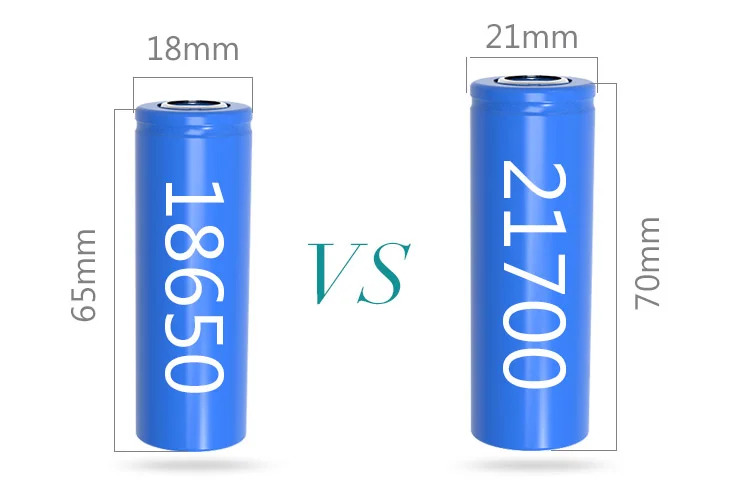
\includegraphics[width=8cm]{images/18650-VS-21700.jpg}
    \caption{18650 VS 21700\cite{tritek_21700_2021}}
    \label{fig:1850VS21700}
\end{figure}


%%TExt als Tabelle

Die Entscheidung zwischen 21700-Zellen und 18650-Zellen für die Batterie-Konstruktion von E-Bikes erfordert eine eingehende wissenschaftliche Analyse verschiedener Faktoren.
Einer der entscheidenden Aspekte ist die energetische Leistung und Kapazität der Zellen.
Die größeren Dimensionen der 21700-Zellen ermöglichen eine höhere Kapazität pro Zelle im Vergleich zu den kleineren 18650-Zellen, dies zu einer potenziell höheren Energiedichte führt und somit die Gesamtkapazität und Reichweite der Batterie positiv beeinflussen kann.\\

Die Verwendung von 21700-Zellen bietet eine Reihe von Vorteilen, die das Preis-Leistungs-Verhältnis im Vergleich zu 18650-Zellen verbessern.
Zum einen sind 21700-Zellen aufgrund ihrer höheren Energiedichte kosteneffizienter, da sie eine größere Kapazität pro Zelle bieten.
Dadurch werden weniger Zellen benötigt, um die gleiche Leistung zu erzielen und führt somit zu einer Einsparung sowohl beim Material als auch bei den Herstellungskosten.
Zudem reduziert die Verwendung weniger Zellen das Risiko von Ausfällen und erfordert weniger Arbeitsaufwand für die Montage und Wartung.\\



Der wichtigste Grund liegt darin, dass durch die höhere Kapazität der 21700-Zellen weniger Zellen benötigt werden.
Dies reduziert nicht nur den Arbeitsaufwand, sondern verringert auch die Ausfallwahrscheinlichkeit bei weniger Zellen.
Im Zuge dieser Untersuchung wurde auch ein defekter Rasenmäher-Akku analysiert und auseinandergenommen.
Dieser konnte die Leistung nicht mehr erbringen, da eine der 18650-Zellen ausgefallen war.
Ein Bild des Rasenmäher-Akkus findet sich im Anhang\ref{fig:20}.\\

Zusammenfassend lässt sich sagen, dass die Verwendung von 21700-Zellen aufgrund ihrer potenziell höheren Kapazität, verbesserten Wärmeableitung und der Möglichkeit, von technologischen Fortschritten zu profitieren, für E-Bike-Batterien vorteilhaft sein könnte.







\subsection{Wahl der Marke}
Die beiden Zelltypen, Samsung und Lishen, unterscheiden sich in mehreren Schlüssel-Parametern, die bei der Entscheidung für die Batterie-Konstruktion eines E-Bikes berücksichtigt werden sollten.\\
Die Samsung-Zellen zeichnen sich durch eine höhere Kapazität von 4900 mAh aus, dies führt potenziell zu einer längeren Betriebsdauer des E-Bikes.
Allerdings liegt der maximale Entladestrom bei 9,8 Amper pro Zelle und kann die Leistungsfähigkeit des Motors ebenso beeinflussen.\\

Im Gegensatz dazu bietet die Lishen-Zelle eine Kapazität von 4000mAh, dies ist etwas niedriger als Samsung.
Allerdings ermöglicht sie einen höheren maximalen Entladestrom von 12 Amper pro Zelle.
Ein zusätzlicher Vorteil könnte sein, dass die Lishen-Zellen preiswerter und somit eine wirtschaftliche Alternative darstellen.\\

In einer Batterie-Konfiguration für E-Bikes spielt die Anzahl der parallel geschalteten Zellen eine entscheidende Rolle für die Entladeleistung.
Sind weniger Zellen parallel geschaltet, bedeutet dies, dass die Gesamtkapazität der Batterie reduziert ist.
Um dennoch die erforderliche Leistung bereitzustellen, muss der Entladestrom pro Zelle erhöht werden.
Es gibt auch Zellen, die einen Entladestrom von 35 Amper liefern. \\

Die Entscheidung zwischen diesen Zellen hängt von den spezifischen Anforderungen des E-Bike-Projekts ab.
Wenn eine längere Reichweite und eine höhere Kapazität priorisiert werden, könnten die Samsung-Zellen die bessere Wahl sein.
Wenn jedoch eine höhere Leistungsfähigkeit des Motors und ein wirtschaftlicher Preis im Vordergrund stehen, könnte die Lishen-Zelle die geeignetere Option sein.
Es ist ratsam, die Projektspezifikationen und das Budget sorgfältig zu prüfen, um die optimale Zell-Wahl zu treffen.\\

Die Entscheidung fiel auf die Lishen-Zellen.
Sie sind am billigsten und es können mehrere parallel geschaltet werden, damit eine höhere Kapazität erreicht werden kann.
Entscheidend ist, dass der Akku genug Leistung zur Verfügung stellen kann.\\

Es werden 13 Zellen in Reihe geschaltet, um 48 Volt zu erreichen, 5 parallel für eine Kapazität von 20 Amperestunden und einen maximalen Entladestrom von 60 Amper.
Siehe Berechnung:~\ref{eq:Strom}.
Die Begründung, weshalb 5 parallel geschaltet werden, ist nachstehend zu sehen: \ref{introduction}

\begin{align}
    A_{\textrm{Batterie}} =& 12 A\cdot 5 = 60 A\\
    V_{\textrm{Batterie}} =& 3.6V \cdot 13 = 46.8V\\
    \textrm{Kapazität} =& 4000mAh \cdot 5 = 20 Ah
    \label{eq:Strom}
\end{align}

In der Abbildung \ref{fig:5} ist der Schaltplan einer solchen Batterie mit BMS dargestellt.



%Hier bin ich stehen geblieben


\section{Battery Management Systems}
%Was ist ein BMS?asdfasdf
Ein entscheidender Aspekt bei der Konstruktion von Lithium-Ionen-Batterien für E-Bikes ist die Wahl des richtigen Battery-Management-Systems (BMS). Dieser Abschnitt erläutert die Funktionen, den Auswahlprozess und die Entscheidungsgrundlagen für die Verwendung eines Balancing-BMS anstelle eines BMS, welches lediglich Überwachungsfunktionen bietet.
Ein BMS ist ein elektronisches System, welches die Leistung und Sicherheit von Lithium-Ionen-Batterien überwacht und regelt.
In seiner Grundfunktion überwacht es Parameter wie Spannung,
Strom, Temperatur und Ladezustand.
Zudem bietet es Schutzmechanismen, um Überladung, Tiefentladung und Überhitzung zu verhindern.\\
Es gibt zwei Haupttypen von BMS: Solche, die lediglich Überwachungsfunktionen bereitstellen, und solche, die auch ein sogenanntes Balancing implementieren.
Balancing bedeutet, dass das BMS aktiv eingreift, um sicherzustellen, dass alle Zellen in der Batterie während des Lade- und Entladevorgangs ähnliche Spannungen aufweisen.\\

%Zweck und Vorteile eines Balancing-BMS:

Die Wahl eines Balancing-BMS für die E-Bike-Batteriekonstruktion basiert auf der Notwendigkeit einer gleichmäßigen Verteilung der Spannung über alle Zellen hinweg, um die Lebensdauer der Batterie zu verlängern und eine optimale Leistung zu gewährleisten.
Im Gegensatz zu einem BMS mit ausschließlich Überwachungsfunktionen interveniert ein Balancing-BMS aktiv, um den Ladungsausgleich zwischen den Zellen sicherzustellen.
Die Variation der Spannung zwischen den Zellen ist problematisch, da sie zu negativen Effekten wie ungleichmäßiger Entladung, Überladung und Tiefenentladung führen kann.
Eine ungleichmäßige Spannungsverteilung kann zu einer ungleichen Alterung der Zellen und vorzeitigem Versagen der Batterie führen.
Durch das aktive Balancing wird vermieden, dass einzelne Zellen aufgrund unterschiedlicher Lade- und Entladezyklen eine Ungleichgewichtssituation erfahren,
dies verbessert was die Batterielebensdauer er verbessert und optimiert die Gesamtleistung des E-Bike-Akkus.\\

Die Entscheidung für ein Balancing-BMS wurde getroffen, um eine maximale homogene Spannungsverteilung zu gewährleisten und sicherzustellen, dass die Batterie effizient, leistungsstark sowie langfristig zuverlässig und haltbar ist.
Hier folgt der Schaltplan der Batterie der mithilfe der gewonnenen Erkenntnisse erstellt wurde \ref{fig:5}.

\begin{figure}[h]
    \centering
    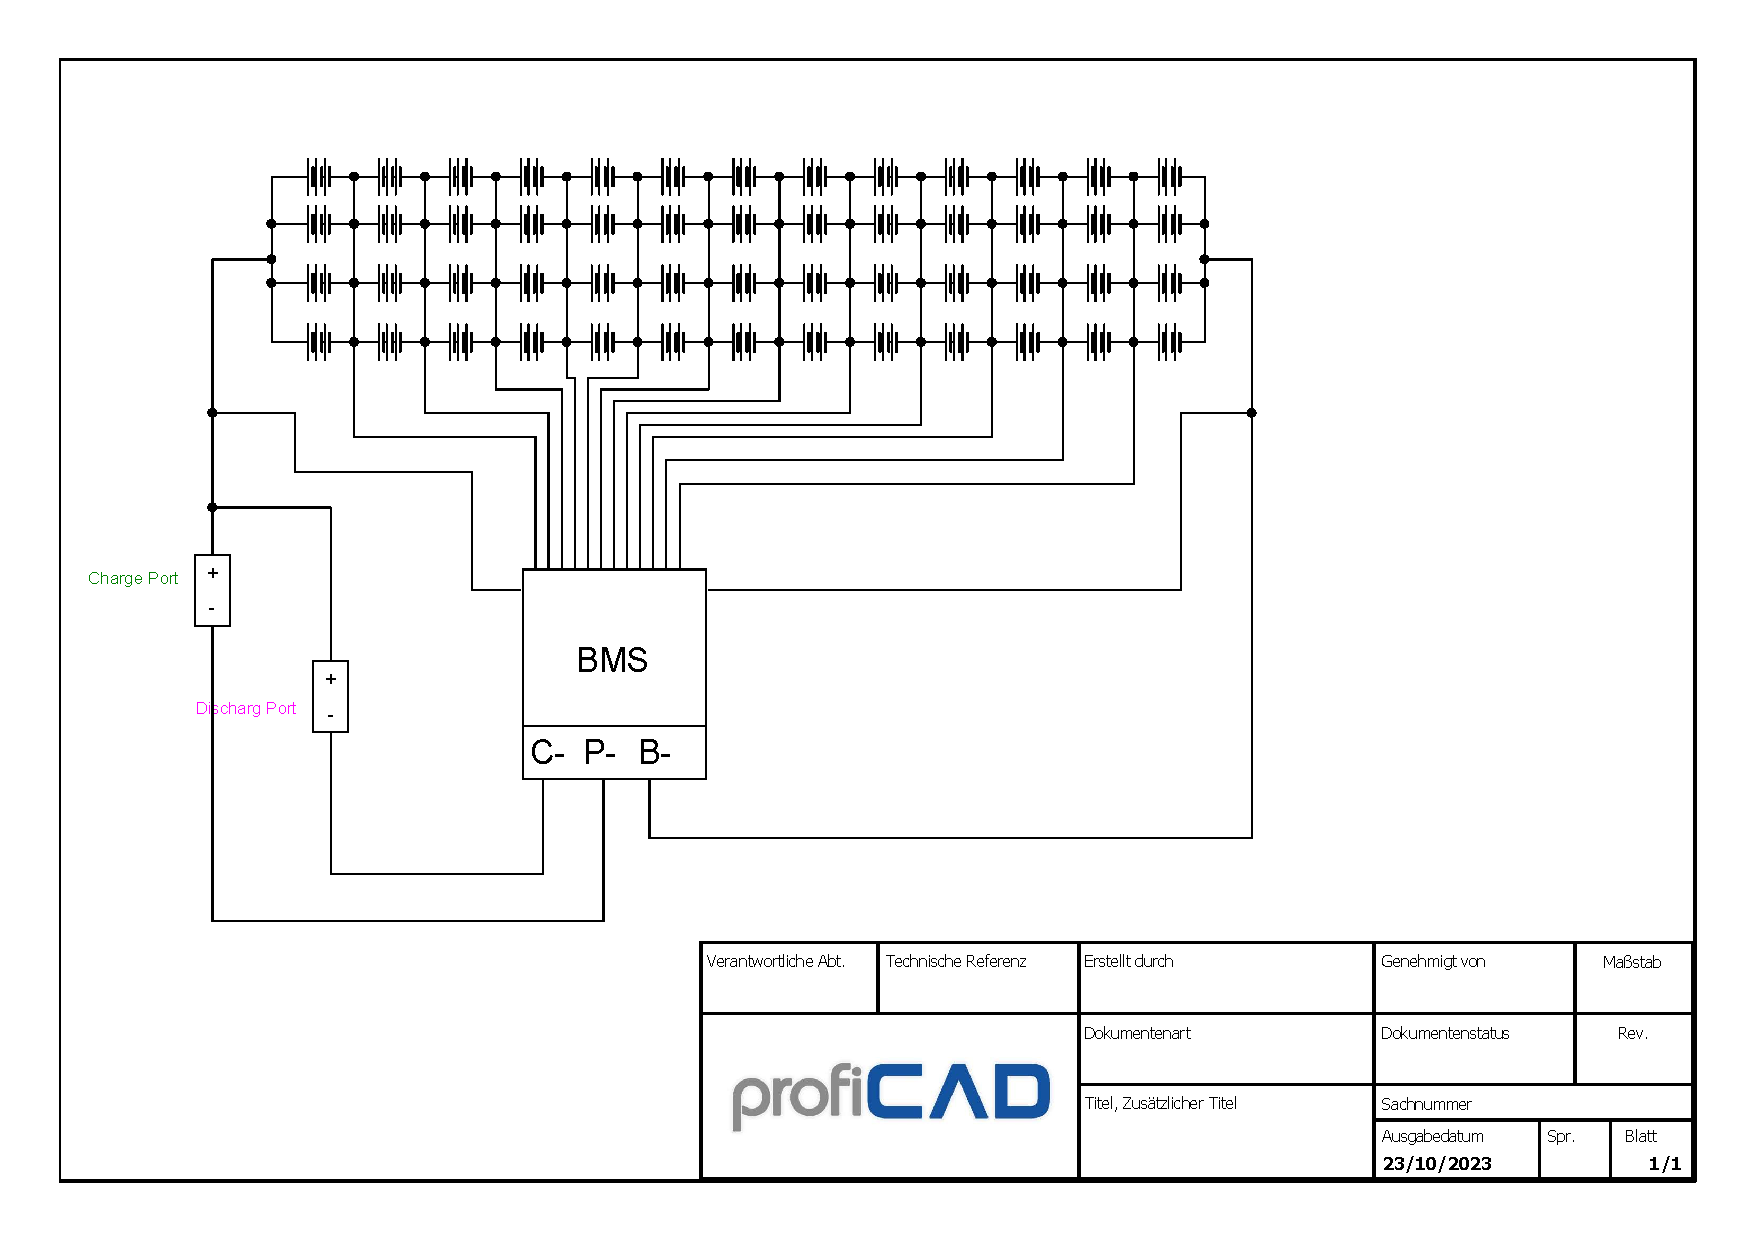
\includegraphics[width=10cm]{images/Schaltplan.pdf}
    \caption{Schaltplan\cite{lorenz_scherrer_selbst_2023}}%
    \label{fig:5}
\end{figure}
Eine größere Version dieser Abbildung ist im Anhang zu finden.\ref{fig:5_1}\\
%Wozu braucht man ein BMS?
Da LLT Power die besten BMS für den Anwendungsfall herstellen, fiel die Entscheidung auf dieses \href{https://www.lithiumbatterypcb.com/product/10s-11s-12s-13s-14s-15s-36v-48v-60v-bms-with-bluetooth-and-pc-communication-120a-constant-current/}{BMS}.

Das BMS verfügt auch über einen Bluetooth Sensor, mit dem es möglich ist die BMS daten in einer App darzustellen\ref{fig:21}.
Hier ist die aktuelle Kapazität, Spannung und Temperatur der Batterie zu erkennen.
Zudem wird auch die aktuelle Differenz unter den Zellen angezeigt und die Spannung jeder Zellenreihe.
\begin{figure}[h]
    \centering
    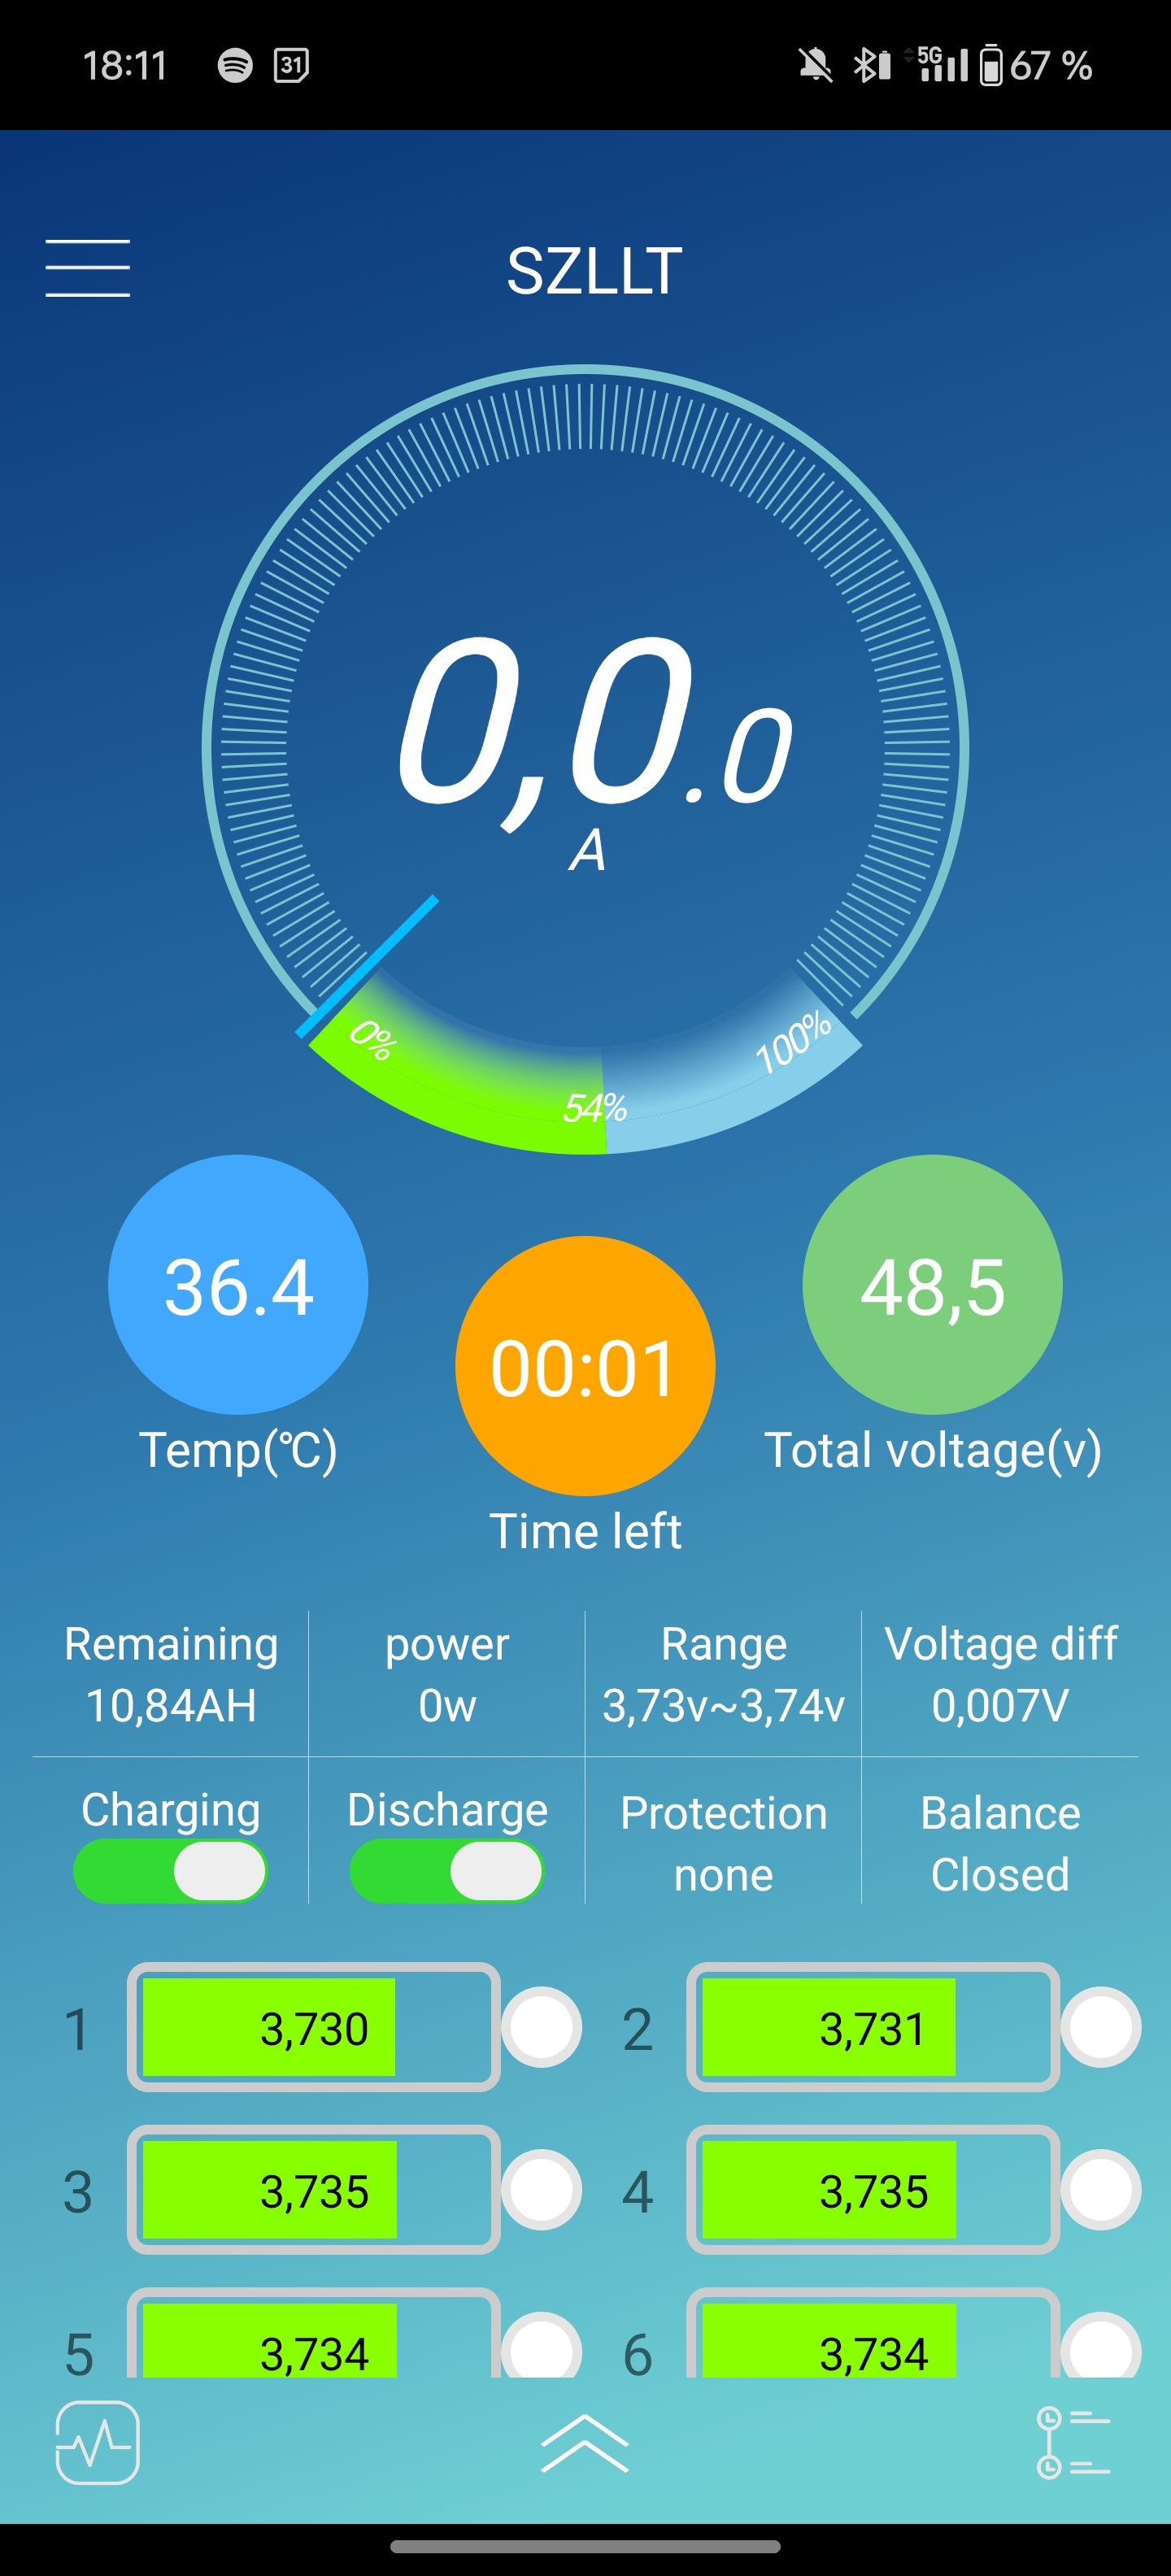
\includegraphics[width=5cm]{images/BMS}
    \caption{BMS-App\cite{lorenz_scherrer_selbst_2023}}%
    \label{fig:21}
\end{figure}
%Wovor schützt ein BMS?
%Für welches BMS wurde ich entschieden?

%Wie schließt man ein BMS an?
%Wie sieht der schaltplan aus?

\section{Verbindung zwischen den Zellen}

Die Verbindung zwischen den Zellen in einer Batterie kann auf verschiedene Weisen hergestellt werden, wobei die gängigsten Methoden das Punktschweißen, das Löten und das Verschrauben sind.
Jede Methode bietet ihre eigenen Vor- und Nachteile.
Die Auswahl hängt von den spezifischen Anforderungen des Batteriedesigns ab.\\

Beim Punktschweißen werden dünnere Drähte oder Metallstreifen direkt an bestimmte Punkte auf den Batteriezellen geschweißt.
Dies geschieht durch kurze elektrische Impulse, die einen Punkt auf der Zelle schmelzen und den Draht oder Streifen daran befestigen.\\

Beim Löten wird ein Lötzinn verwendet, um die Verbindungen zwischen den Zellen und den Verbindungselementen herzustellen.
Dies kann mit einem Lötkolben erfolgen, der das Lötzinn schmilzt und es an Ort und Stelle hält, wenn es abkühlt.\\

Diese Methode beinhaltet das Anbringen von Metallfassungen an den Enden der Batteriezellen, die dann miteinander verschraubt werden.
Die Fassungen dienen als Anschlusspunkte für die Verbindungselemente.\\

\subsection{Löten vs. Punktscheißen}
Die Wahl der geeigneten Methode zur Verbindung von Batteriezellen ist entscheidend für die Leistung, Sicherheit und Mobilität eines E-Bike-Batteriesystems.
Angesichts der spezifischen Anforderungen und Einschränkungen wurde die Entscheidung getroffen, nur Löten und Punktschweißen in Betracht zu ziehen, wobei die Methode der mechanischen Verbindung mit Fassungen ausgeschlossen wurde.\\

%Beschränkungen der mechanischen Verbindung:
Die Methode der mechanischen Verbindung mit Fassungen wurde aus mehreren Gründen ausgeschlossen.
Die schwere und kostspielige Natur dieser Methode erwies sich als unpraktisch für die Anzahl der Zellen in einer E-Bike-Batterie.
Darüber hinaus war die mobile Verwendung des E-Bikes ein entscheidender Faktor, und eine zu komplexe mechanische Verbindung hätte die Tragbarkeit des Systems erheblich beeinträchtigt.\ref{fig:2}\\
%Bild von meschanischer Fassung
\begin{figure}[h]
    \centering
    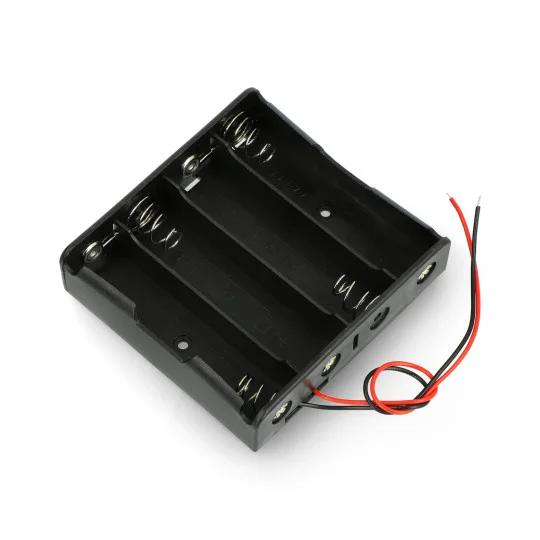
\includegraphics[width=8cm]{images/korb-fur-4-18650-akkus-reihenschaltung.png}
    \caption{ Fassung für 18650 Batterie\cite{noauthor_korb_2024}}%
    \label{fig:2}
\end{figure}


%Auswahl zwischen Löten und Punktschweißen:
Nach Ausschluss der mechanischen Verbindung blieben Löten und Punktschweißen als die beiden geeigneten Optionen für die Verbindung der Batteriezellen.
Obwohl beide Methoden ihre Vor- und Nachteile haben, wurde eine fundierte Entscheidung getroffen, um den spezifischen Anforderungen gerecht zu werden.\ref{fig:3}\\
%Bild vom Punktschweißen
\begin{figure}[ht]
    \centering
    \includegraphics[width=8cm]{images/Punktschweißen_beispiel.jpg}
    \caption{ Punktgeschweißte Verbindung\cite{lorenz_scherrer_selbst_2023}}%\cite{selbst Experiment}
    \label{fig:3}
\end{figure}

%Löten als kosteneffiziente Option
Löten ist die kosteneffizientere Option mit dem geringen Beschaffungsaufwand, da es weniger spezielle Ausrüstung erfordert und leichter zugänglich ist.
Die Einfachheit des Lötens ermöglichte eine effiziente Materialbeschaffung und eine schnellere Umsetzung.
Obwohl Löten die Batterie durch die Wärmeentwicklung belasten kann und sie weniger Stabil ist.
Diese Vermutung muss durch einen Test geprüft werden, da die andere Option nicht ohne weiteres zugänglich ist.\ref{fig:4}\\
% Bild vom Löttest
\begin{figure}[ht]
    \centering
    \includegraphics[width=8cm]{images/Löten.png}
    \caption{ Verbindung Löten\cite{lorenz_scherrer_selbst_2023}}
    \label{fig:4}
\end{figure}

%Fazit
Das Punktschweißen der Batteriezellen wurde als bevorzugte Methode ausgewählt, da Löten aufgrund seiner Instabilität und des erhöhten Platzbedarfs mechanisch weniger praktikabel war.
Die Auswahl der geeigneten Verbindungsmethode für Batteriezellen ist von entscheidender Bedeutung für Leistung, Sicherheit und Mobilität eines E-Bike-Batteriesystems.
Angesichts der spezifischen Anforderungen und Einschränkungen erwies sich das Punktschweißen als die effizienteste Lösung, während die mechanische Verbindung mit Fassungen aus mehreren Gründen ausgeschlossen wurde.
Die komplexe Natur und der hohe Platzbedarf der mechanischen Verbindung wären unpraktisch für die Anzahl der Zellen gewesen und hätten die Tragbarkeit des Systems beeinträchtigt.
Nachdem die mechanische Verbindung ausgeschlossen war, blieben Löten und Punktschweißen als die beiden geeigneten Optionen für die Verbindung der Batteriezellen.
Löten erwies sich als kosteneffizienter, erforderte jedoch einen Test, um die Stabilität zu bestätigen.
Punktschweißen hingegen bot eine Standardlösung mit hoher Stabilität und geringerer Wärmeentwicklung auf den Batterien.
Insgesamt wurde das Punktschweißen aufgrund seiner Effizienz und Zuverlässigkeit als bevorzugte Methode für die Verbindung der Batteriezellen für das E-Bike-Batteriesystem gewählt.\\




% Löten 
% -schnell
% -nicht stabil
% -es wurde ein test gemacht hier bild ein blenden
% -wenn nicht stabil hocher winderstand
% -Hitze auf den Batterien genau gefahren kann in die Luft gehen
% -Sicherung doch dünne drähte
% -mehr platz für 
% -Versuchsbeschreibung in einer Wissenschaftlichen Arbeit

% Punktzuschweißen
% -standard
% -sehr stabil
% -geringer Hitze auf den Batterien
% -

% Meschanisch verbinden
% -am besten und am sicherseten
% -kosten intensive
% -schwer viel platz wird gebraucht

\section{Punktschweißgerät}
%Wie funktioniert schweißen?

Das Punktschweißen ist ein gängiges Widerstandsschweißverfahren, das zur Verbindung von einem Blech und einer Zelle ohne den Einsatz von Zusatzwerkstoffen verwendet wird.
Dabei werden die zu verbindenden Werkstücke durch die Erzeugung von Wärme an der Kontaktstelle verschmolzen und zu einer festen Verbindung vereint.
Das Funktionsprinzip des Punktschweißens beruht auf der Nutzung elektrischen Stroms, um die erforderliche Wärmeenergie zu erzeugen und die Werkstücke zu verbinden.



\subsection{Erforderlicher Strom für das Punktschweißen}

Der für das Punktschweißen benötigte Strom hängt von verschiedenen Faktoren ab, darunter die Materialien der Werkstücke, ihre Dicke und die gewünschte Schweißqualität.
Typischerweise liegt die erforderliche Stromstärke im Bereich von mehreren Hundert bis Tausend Ampere.\\

Die hohe Stromstärke ist notwendig, um ausreichend Wärmeenergie an der Schweißstelle zu erzeugen und die Bleche lokal aufzuschmelzen.
Niedrigere Ströme würden nicht genügend Wärme erzeugen, um die erforderliche Schmelztemperatur zu erreichen.\\

Insgesamt ist das Punktschweißen ein effizientes Verfahren zur Herstellung von festen Verbindungen zwischen Blechen.
Es erfordert einen geeigneten elektrischen Strom, um die erforderliche Wärmeenergie zu erzeugen und die Werkstücke erfolgreich zu verschweißen.\\

%Wie funktioniert ein Punktscheißgerät?


\subsection*{ Transformator}
%Man braucht einen Transformator?

Ein Transformator wird beim Punktschweißen verwendet, um die erforderliche Stromstärke und Spannung für den Schweißprozess bereitzustellen.\\

%wie funktioniert einen transformator? %Wie funktioniert die Transformator formel?
Ein Transformator ist ein elektrisches Gerät, das verwendet wird, um die Spannung von Wechselstrom (AC) zu ändern.
Es besteht aus zwei Spulen, die eng miteinander gekoppelt sind, aber elektrisch isoliert voneinander sind.
Diese Spulen sind als Primär- und Sekundärwicklung bekannt.\\

%Abbildung von einen Transformator

Das Funktionsprinzip eines Transformators basiert auf elektromagnetischer Induktion.
Wenn Wechselstrom durch die Primärwicklung fließt, erzeugt er ein wechselndes Magnetfeld um die Spule herum.
Dieses Magnetfeld induziert eine Spannung in der Sekundärwicklung gemäß den Prinzipien der elektromagnetischen Induktion von Faraday.\\

%Wie muss man den transformator verändern? %Wie muss der Transformator gewickelt werden? 

Die Verhältnisse der Windungen in der Primär- und Sekundärwicklung bestimmen die resultierende Spannungsumwandlung.
Wenn die Anzahl der Windungen in der Sekundärwicklung größer ist als die in der Primärwicklung, wird die Spannung im Verhältnis erhöht (Step-Up-Transformator).
Wenn die Anzahl der Windungen in der Sekundärwicklung kleiner ist als die in der Primärwicklung, wird die Spannung im Verhältnis reduziert (Step-Down-Transformator).\\

%Wo bekommt man einen transformator her?


Ein Mikrowellen-Transformator eignet sich sehr gut für den Bau eines Punktschweißgeräts.


Um herauszufinden, wie der sekundäre Block gewickelt werden muss, kann die Transformator formel verwendet werden.\ref{eq:3}

Transformator Formel:
\begin{align}%
        \frac{U_s}{U_p} &= \frac{N_s}{N_p}\\
        \frac{U_s}{U_p}\cdot N_p &= N_s \\
        \frac{I_s}{I_p} &=\frac{N_p}{N_s}\\
        \frac{I_p}{I_s} \cdot N_p = N_s &= \frac{16A}{800A}\cdot 224 \approx 4.48
        \label{eq:3}
\end{align}
        
        \begin{conditions*}
            U_p  &  Spannung am primären Block\\
            U_s  &  Spannung am sekundären Block $\approx 4V$ \\
            I_p  &  Stromstärke am primären Block = 16A\\
            I_s & Stromstärke am sekundären Block\\
            N_p & Wicklungen primären Block = $16\cdot14=224$\\
            N_s & Wicklungen sekundären Block\\
        \end{conditions*}




\subsubsection*{Demontage des Transformators}
Die Sekundärwicklung wurde mithilfe einer Maschine durchgesägt, um die Sekundärwicklung so zu wickeln, wie oben berechnet, siehe Formel\ref{eq:3}.
Beim Durchsägen wurde die primäre Wicklung beschädigt, siehe Bild\ref{fig:35}, weshalb ein neuer Transformator beschafft werden musste.
Der Block muss auf einer Seite mit einer Stahlsäge durchtrennt werden und dann herausgeschlagen werden.
Bei dem zweiten Transformator wurde die sekundäre Wicklung ebenfalls beschädigt, was eine Lötarbeit erforderte.
Dabei musste sorgfältig darauf geachtet werden, die Isolierung der Wicklungen zu entfernen und die Drahtenden wieder zu verbinden.



\subsubsection*{Aufbau des Punktschweißgeräts}
Ein Holzblock diente als Basis und Halterung für den Transformator.
Der Block wurde so modifiziert, dass er den Transformator sicher hielt und gleichzeitig eine einfache Handhabung ermöglichte.
Es wurde ein 5mm dicker Kupferdraht angespitzt die den Kontakt mit dem Nickelband herstellen wird, siehe Bild\ref{fig:23}.

\begin{figure}[ht]
    \centering
    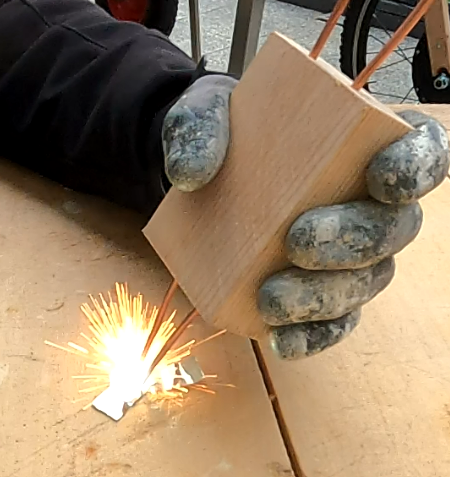
\includegraphics[width=8cm]{images/Funke}
    \caption{Punktschweißen von zwei Nickelstreifen\cite{lorenz_scherrer_selbst_2023}}
    \label{fig:23}
\end{figure}

\subsubsection*{Elektrische Verbindungen und Steuerung}
Um den Schweißvorgang zu steuern, wurden verschiedene Methoden in Betracht gezogen.
Standardlösungen wie ein spezieller Controller wurden aufgrund der Kosten und Komplexität verworfen.
Stattdessen wurde ein einfacher Push-Button-Schalter(Lichttaster) verwendet, um den Stromkreis kurzzeitig zu schließen und den Schweißvorgang auszulösen.
Hier oben rechts im Bild zu sehen\ref{fig:22}.


\begin{figure}[ht]
    \centering
    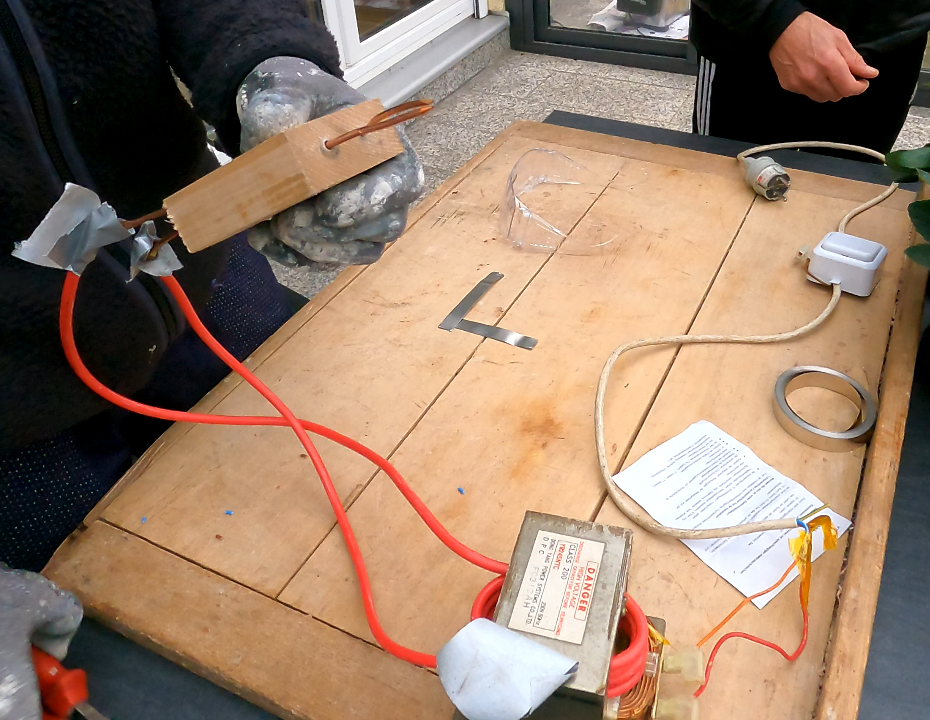
\includegraphics[width=8cm]{images/Transformator und Punktschweißgerät}
    \caption{ Punktschweißgerät\cite{lorenz_scherrer_selbst_2023}}
    \label{fig:22}
\end{figure}




%Bilder vom entfernen des Blocks

%Weitere Probleme?

%Versuchs beschreibung in einer Wissenschaftlichen arbeit?
%Neuer Transformator?





%Wie schaltet man das Punktschweißgerät ein?
%Controller
%schalter
%Taster

\section{Konstruktion der Batterie}

Es wurde beschlossen, die Zellen mit doppelseitigem Klebeband anstatt mit Heißkleber zu verbinden.

%Bilder von der Batterie

Anschließend wurden alle Zellen punktverschweißt, sowohl in Reihe als auch parallel geschaltet.
Die Anschlüsse des Batteriemanagementsystems (BMS) wurden gemäß dem Blockschaltbild \ref{fig:5_1} an die jeweilige Zellreihe angeschlossen.
Nach Abschluss dieser Schritte wurde der Batteriepack mit einer Umwicklung aus Katonasch und Kaptontape isoliert.
Diese Maßnahme diente dazu, die Zellen vor äußeren Einflüssen zu schützen und potenzielle Kurzschlüsse zu vermeiden.
Nach der Isolierung konnte der Batteriepack erfolgreich mit einem Ladegerät geladen werden.


